
\documentclass[12pt]{article}
\usepackage[margin=1in]{geometry}
\usepackage[pdftex]{graphicx}
\usepackage{multirow}
\usepackage{setspace}
\usepackage{enumitem}
\pagestyle{plain}
\setlength\parindent{0pt}

\begin{document}

% Course information
\begin{tabular*}{\textwidth}{l @{\extracolsep{\fill}} r}
  & \multirow{3}{*}{
\includegraphics[height=1.0in]{logo.jpg}} \\
  \large Experimental Techniques & \\
  \large Winter Quarter 2019 & \\
  \large Physics 80 & \\
\end{tabular*}
\vspace{10mm}

% Professor information
\begin{tabular}{ l l }
  \multirow{6}{*}{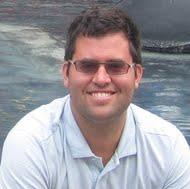
\includegraphics[height=1.25in]{mike.jpg}} & \\
  & \\
  & \large Michael Mulhearn \\
  & \large mulhearn@physics.ucdavis.edu \\
  & \large Physics 317 \\
  & \\
\end{tabular}
\vskip 0.5cm
\noindent
%\textbf {Lectures:} M,W 11:00-11:50 PM in Rm. 285 Physics
\textbf {Lectures:} M,W 11:00-11:50 PM in Rm. 152 Roessler (moved from Rm. 285 Physics)
\begin{tabbing}
\hspace*{3em}\= \hspace*{5em} \= \kill % set the tabbings
\textbf {Lab:}    \> Section 1: \>  M 12:10-2:40 PM in Rm. 152 Roessler \\
%                        \> Section 2: \> W 3:10-6:00 PM in Rm. 152 Roessler \\
\end{tabbing}

\noindent
\textbf {Text:}  Online lecture notes at {\tt https://www.scipy-lectures.org} plus
lecture notes on RLC circuits and Data Analysis. \\

\noindent
\textbf{Office Hours:} M 3:00-4:00 PM in Physics 317 \\

\noindent
\textbf{Lab Instructor:} Samuel Heppelmann, sheppelmann@ucdavis.edu \\

\noindent
\textbf{Quizzes:}  There will be occasional low-stakes single-problem quizzes during lecture.\\

\noindent
\textbf{Final Exam:} Wed, March 20 at 1:00 pm in 285 Physics \\

\noindent
\textbf{Homework:} There will be approximately five homework
assignments, based on the lecture material.  Do not post the problems
to internet forums.  To minimize the effectiveness of cheating,
homework scores will be based solely on whether a legitimate attempt
was made.  The best way to prepare for the exams and the quizzes is to
solve problems yourself or within a study group.  Always be prepared
to explain your work.\\

\noindent
\textbf {Course Description:}  This course is an introduction to experimental laboratory techniques and data analysis.  Laboratory techniques include electronics circuits and optical systems and related test equipment.  Data analysis based on scientific python includes statistical and systematic analysis, curve fitting, and noise.\\

\noindent
\textbf {Lab Safety:} 
You should complete the online course for Electrical Safety at \\
{\tt http://safetyservices.ucdavis.edu/training/electrical-safety}.\\


\noindent
\textbf {Labs:} 
You are expected to attend every lab session.  The TA will take attendance at the start of each lab, therefore, if you arrive late, you should check in with the TA.   Most labs have one or more sign-off points where you are expected to show the TA your result.  If time permits, the TA may ask a questions of each lab partner.  For example, to describe the purpose of a particular line of code.  When appropriate, you may be assigned a grade for neatness of your experimental setup and/or code.\\

There is no opportunity to make-up labs that are missed or not completed during the designated time.  Instead, your worst two lab scores will be dropped from your final grade.  \\

\noindent
\textbf {Pre-Lab Calculations:} 
If assigned, pre-lab calculations are due at the start of lab.  They will be left at the front of the class in case you need to consult them during lab.\\

\noindent
\textbf {Lab Reports:} 
Most scientist employ a mixture of handwritten and digital logbooks.  Quick notes and sketches about procedures, calculations, and the results of simple measurements are often most conveniently handwritten.  But data collection and detailed analysis are done entirely on a computer.\\

Each student will maintain a personal handwritten logbook (For this
class, any bound notebook will do, including spiral bound, but not
loose leaf paper) in order to record notes on the procedure, as well
as record observations and simple measurements.  The handwritten
logbook will remain in the lab to be graded periodically and eliminate
the risk of being lost.  Extensive analysis and final plots will be
submitted online.  Place the names of all lab partners in the top cell
of the notebook, then print it as a PDF and upload to Canvas at the
end of lab.  One submission per team.\\

\noindent
\textbf {Tentative Course Outline}:
This is the first time this course has been offered, so the topics and schedule may be adjusted while the course is in progress.

\begin{table}[h!]
\normalsize % The size of the table text can be changed depending on content. Remove if desired.
\begin{tabular}{ lllll }
\hline
\textbf{Week} & \textbf{Dates} & \textbf{Lecture} & \textbf{Lab} \\
\hline
1 & 7 Jan & Introduction & (no lab) \\
   & 9 Jan & Scientific Python & Plotting\\
\hline
2 & 14 Jan & RLC Circuits & DC Circuits \\
  & 16 Jan & & Thevenin Equivalent Circuits \\
\hline
3 & 23 Jan & & Time Varying Signals \\
\hline
4 & 28 Jan & & RC amd RL Transient Signals \\
   & 30 Jan &  &  Passive Filters and Resonance \\
\hline
5 & 4 Feb & Distributions & Catch Up \\
   & 6 Feb & & Distributions \\
\hline
6 & 11 Feb & Uncertainties & Geiger Counter \\
   & 13 Feb & & Central Limit Theorem and Uncertainties \\
\hline
7 & 20 Feb & The Diode & The Diode\\
\hline
8 & 25 Feb & Analysis & Curve Fitting \\
   & 27 Feb & & Planck's Constant \\
\hline
9 & 4 Mar & & Speed of Light \\
   & 6 Mar & & TBA \\
\hline
10 & 11 Mar & & Muon Lifetime\\
   & 13 Mar & & TBA\\
\hline
\end{tabular} 
\end{table}

\end{document}

